\documentclass[wip, topology]{bsteffan-lecturenotes}

\usetikzlibrary{math, matrix, patterns, patterns.meta}

\addbibresource{references.bib}

\colorlet{knowngray}{darkgray!70}

\DeclareNamedOperator{Stab}
\DeclareNamedOperator{gr}
\DeclareNamedOperator{sk}

\tikzset{
	spectral sequence/.cd,
	axis/.style = {
		thick,
		->,
		font = \footnotesize
	},
}

\course{Algebraic Topology \uppercase\expandafter{\romannumeral 1\relax}}
\subtitle{The Serre Spectral Sequence, Characteristic Classes, and Bordism}
\lecturer{Prof. Dr. Markus Hausmann}
\assistant{Dr. Elizabeth Tatum}
\author{Ben Steffan}

\begin{document}
\maketitle
\tableofcontents
\listoflectures

\setcounter{section}{-1}
\section*{About These Notes}
This document encompasses lecture notes for the course \makeatletter\@course\makeatother\ taught in the winter term of 2023/24 at the University of Bonn by \makeatletter\@lecturer\makeatother.
The assistant is \makeatletter\@assistant\makeatother.

These notes are for private use. 
They are \strong{not} official lecture notes endorsed by the lecturer.
As such, errors and inaccuracies that persist are generally my own (unless proven otherwise).

This document is not a character-for-character transcript of the lecture.
Changes to form (though generally not to content) have been made to improve readability of these notes as a document.
In particular, I have taken the liberty to make adjustments to notation here and there to more closely align with my personal tastes and opinions.
At points, I have added additional context, explanations, computations, and so on.
These are clearly marked to that effect, although smaller changes and in-text additions (such as citations) are not.

\subsection*{Formatting}
This document has hyperlinks: References, footnote marks, table-of-contents entries and so on are linked and can be clicked to take you to the corresponding item.
Except for footnote marks, which remain black, all such links are highlighted in either \textcolor{linkcol}{orange} or \textcolor{citecol}{violet}. 
\textcolor{highlightcol}{Red} is used to highlight certain items formulas and diagrams.
The colors \textcolor{definitioncol}{green}, \textcolor{exercisecol}{blue}, and \textcolor{theoremcol}{red} are used as border colors to higlight definitions, exercises, and theorems, propositions, lemmas, etc., respectively.
\textcolor{knowngray}{Gray} is used to convey known or secondary information in formulas and diagrams from place to place.

Demarcations for lecture dates are placed in the righthand margin.

\section{Informal Introduction}\lecture{09.10.23}
\begin{note}
	We omit the coefficient group $\Z$ from notation in (co)homology as well as basepoints where they are of no particular relevance in homotopy groups.
\end{note}
One of the big goals of homotopy theory is to compute
\[
	[X, Y]_* = \{\text{basepoint-preserving continuous maps } X \to Y\} / \text{homotopy}
\]
for $X$ and $Y$ pointed CW-complexes.
CW-complexes are built out of spheres, so the building blocks are the sets
\[
	[S^n, S^k]_* = \pi_n(S^k, *)
\]
For $n \geq 1$ these are groups and abelian if $n \geq 2$.
We know that\textellipsis{}
\begin{itemize}
	\item $\pi_n(S^k) = 0$ for $n < k$ by cellular approximation, cf. \cite[Corollary 4.9]{hatcher_algebraic_2002},
	\item $\pi_n(S^n) \isom \Z$ by the Hurewicz theorem (cf. \cite[Theorem 4.32]{hatcher_algebraic_2002}) and $H_n(S^n) \isom \Z$: 
		If $X$ is an $(n - 1)$-connected CW-complex ($n > 1$), then there is an isomorphism $\pi_n(X) \xto{\isom} H_n(X)$, 
	\item $\pi_k(S^1) = 0$ for $k \geq 2$ via covering space theory: The universal cover of $S^1$ is $\R$ which is contractible, 
	\item $\pi_3(S^2) \neq 0$ since the attaching map of the 4-cell for $\CP^2$ is a map $\eta\colon S^3 \to S^2 = \CP^1$; if $\eta$ was nullhomotopic, then $\CP^2$ would be homotopy equivalent to $S^2 \vee S^4$ which contradicts the ring structure on $H^*(\CP^2) \isom \Z[x] / x^3$, and that
	\item The sequence
		\begin{equation*}
			\pi_k(S^n) \to \pi_{k + 1}(S^{n + 1}) \to \pi_{k + 2}(S^{n + 2}) \to \cdots
		\end{equation*}
		always stabilizes by the \emph{Freudenthal suspension theorem} (see \cite[Corollary 4.24]{hatcher_algebraic_2002}).
\end{itemize}
To go beyond this, we will need a new tool, the \emph{Serre spectral sequence}.
To motivate its usefulness for this question, consider the following strategy:
There exists a map $f\colon S^2 \to K(\Z, 2)$ which induces an isomorphism $f_*\colon \pi_2(S^2) \xto{\isom} \pi_2(K(\Z, 2)) \isom \Z$.
We can take its homotopy fibre $H \coloneq \hofib(f_*)$; there is then a fibre sequence $H \to S^2 \xto{f} K(\Z, 2)$ and thus a long exact sequence\footnote{The groups in \textcolor{knowngray}{gray} are assumed known. The groups and properties in \textcolor{col05}{red} follow from those in gray.}
\begin{equation*}
	\begin{tikzpicture}[commutative diagrams/.cd, every diagram, row sep = large]
		\matrix[matrix of math nodes, name = m, commutative diagrams/every cell] {
				& \cdots & \pi_4(K(\Z, 2)) \\
			\pi_3(H) & \pi_3(S^2) & \pi_3(K(\Z, 2)) \\
			\pi_2(H) & \pi_2(S^2) & \pi_2(K(\Z, 2)) \\
			\pi_1(H) & \pi_1(S^2) & \pi_1(K(\Z, 2)) & 0 \\
		};
		\path[commutative diagrams/.cd, every arrow, every label]
			(m-1-2) edge (m-1-3)
			(m-1-3) edge[rounded corners, to path = {
				-- ([xshift = 1em] \tikztostart.east)
				|- ($(m-1-2)!0.5!(m-2-2)$) \tikztonodes
				-| ([xshift = -2ex] \tikztotarget.west)
				-- (\tikztotarget)
			}] (m-2-1)
			(m-2-1) edge["{\color{highlightcol}\isom}"] (m-2-2) 
			(m-2-2) edge (m-2-3)
			(m-2-3) edge[rounded corners, to path = {
				-- ([xshift = 1em] \tikztostart.east)
				|- ($(m-2-1)!0.5!(m-3-1)$) \tikztonodes
				-| ([xshift = -2ex] \tikztotarget.west)
				-- (\tikztotarget)
			}] (m-3-1)
			(m-3-1) edge (m-3-2) 
			(m-3-2) edge["$f_*$", "$\isom$"'] (m-3-3)
			(m-3-3) edge[rounded corners, to path = {
				-- ([xshift = 1em] \tikztostart.east)
				|- ($(m-3-1)!0.5!(m-4-1)$) \tikztonodes
				-| ([xshift = -2ex] \tikztotarget.west)
				-- (\tikztotarget)
			}] (m-4-1)
			(m-4-1) edge (m-4-2) 
			(m-4-2) edge (m-4-3)
			(m-4-3) edge (m-4-4);
		% don't want our labeling nodes to be the usual node grid distance away
		% better to set this via scope than to either pass it to each \node separately or set it for the whole picture
		\begin{scope}[node distance = -5.25pt, knowngray] 
			\node[below = of m-1-3] {$0$};
			\node[below = of m-2-3] {$0$};
			\node[below = of m-3-1, highlightcol] {$0$};
			\node[below = of m-4-1, highlightcol] {$0$};
			\node[below = of m-4-2] {$0$};
			\node[below = of m-4-3] {$0$};
		\end{scope}
	\end{tikzpicture}
\end{equation*}
Hence, $H$ is 2-connected and $\pi_n(H) \to \pi_n(S^2)$ is an isomorphism for all $n \geq 3$.
By the Hurewicz theorem, the following diagram commutes:
\begin{equation*}
	\begin{tikzcd}
		\pi_3(H)
				\ar[r, "\isom"]
				\ar[dr, swap, "\isom"]
			& H_3(H)
		\\
			& \pi_3(S^2)
				\ar[u, swap, "\isom"]
	\end{tikzcd}
\end{equation*}
If we had a way to compute $H_*(H)$ from $H_*(S^2)$ (the computation of which is easy) and $H_*(K(\Z, 2))$ (which is known), we could compute $\pi_3(S^2)$ this way!

\subparagraph{Upshot}
It would be useful to have a tool which relates the homology groups of the three terms in a fibre sequence.
This will also help us to compute $\pi_n(S^k)$ in other ways (for example, we will show that $\pi_n(S^k)$ is finite unless $n = k$ or $n = 2k - 1$ and $k$ is even).
Furthermore, the Serre spectral sequence will allow us to compute the (co)homology of spaces like $\Uni(n)$, $\SU(n)$, $\Omega S^n$, $K(\Zn{2}, n)$ and (re)prove structural theorems like the Hurewicz theorem, the Freudenthal suspension theorem, Thom isomorphisms, and more.

So, given a fibre sequence $F \to Y \to X$, what could the relationship between the homology groups of $F$, $Y$ and $X$ be?
\begin{example}
	Consider the easiest case $F \to X \times F \xto{\pr_X} X$ (a \emph{trivial fibration}).
	Then the Alexander-Whitney map induces an isomorphism $H_n(X \times F; \Z) \xto{\isom} \bigdsum_{p + q = n} H_p(X, H_q(F))$, so it computes the homology of the total space in terms of the homology of $X$ and $F$.
\end{example}
\begin{example}
	Consider the Hopf fibration $S^1 \to S^3 \xto{\eta} S^2$.
	We can compute
	\begin{equation*}
		\renewcommand{\arraystretch}{1.1}
		\begin{tabular}{r|c|c}
			$n$ 		& $H_n(S^3; \Z)$ 	& $\bigdsum_{p + q = n} H_p(S^3; H_q(S^1; \Z))$ \\\hline
			0 			& $\Z$ 				& $\Z$ \\
			1 			& $0$				& $\Z$ \\
			2 			& $0$				& $\Z$ \\
			3 			& $\Z$ 				& $\Z$ \\
			4 			& $0$				& $0$ \\
			$\vdots$ 	& $\vdots$			& $\vdots$
		\end{tabular}
	\end{equation*}
	so $\bigdsum_{p + q = n} H_p(S^3; H_q(S^1; \Z))$ is in some sense \enquote{too big} to describe $H_n(S^3; \Z)$ in degrees $n = 1, 2$.
	Note, however, that we can consider a \enquote{2-step filtration} $S^1 \subseteq S^3$ which satisfies $\tilde{H}_n(S^3 / S^1; \Z) \isom \Z$ if $n = 2, 3$ and $0$ else.
	Then
	\begin{equation*}
		\renewcommand{\arraystretch}{1.1}
		\begin{tabular}{r|c}
			$n$ & $H_n(S^1; \Z) \dsum \tilde{H}_n(S^3 / S^1; \Z)$ \\\hline
			0 	& $\Z$ \\
			1 	& $\Z$ \\
			2 	& $\Z$ \\
			3 	& $\Z$ \\
			4 	& 0 \\
			$\vdots$ 	& $\vdots$ \\
		\end{tabular}
	\end{equation*}
	This does not agree with $H_3(S^3; \Z)$ because in the long exact sequence
	\begin{equation*}
		\begin{tikzcd}[row sep = large]
			\cdots 
					\ar[r]
				& H_3(S^3; \Z)
					\ar[r]
				& \tilde{H}_3(S^3 / S^1; \Z)
					\ar[dll, rounded corners, swap, "\del", to path = {[pos = 1]
						-- ([xshift = 1em] \tikztostart.east)
						|- ($(\tikzcdmatrixname-1-2)!0.5!(\tikzcdmatrixname-2-2)$) \tikztonodes
						-| ([xshift = -2ex] \tikztotarget.west)
						-- (\tikztotarget)
					}]
			\\
			H_2(S^1; \Z)
					\ar[r]
				& H_2(S^3; \Z)
					\ar[r]
				& \tilde{H}_2(S^3 / S^1; \Z)
					\ar[dll, rounded corners, swap, "\del", "{\color{highlightcol}\isom}"', to path = {[pos = 1]
						-- ([xshift = 1em] \tikztostart.east)
						|- ($(\tikzcdmatrixname-2-2)!0.5!(\tikzcdmatrixname-3-2)$) \tikztonodes
						-| ([xshift = -2ex] \tikztotarget.west)
						-- (\tikztotarget)
					}]
			\\
			H_1(S^1; \Z)
					\ar[r]
				& H_1(S^3; \Z)
					\ar[r]
				& \cdots
		\end{tikzcd}
	\end{equation*}
	the boundary map $\tilde{H}_2(S^3 / S^1; \Z) \to H_1(S^1; \Z)$ is an isomorphism.
	Hence, $H_1(S^1; \Z)$ does not contribute to $H_1(S^3; \Z)$ and $\tilde{H}_2(S^3 / S^1; \Z)$ does not contribute to $H_2(S^3; \Z)$.
\end{example}
It turns out that something similar holds for all fibre sequences $F \to Y \to X$: 
There exists a filtration on $C_*(Y; \Z)$
\begin{equation*}
	F_0 \subseteq F_1 \subseteq \cdots \subseteq F_m \subseteq \cdots \subseteq C_*(Y; \Z)
\end{equation*}
of chain complexes such that $H_{p + q}(F_p / F_{p - 1}) \isom C^{\text{cell}}_p(X; H_q(F; \Z))$.
To understand $H_*(Y; \Z)$, one needs to understand the cancellations in the associated long exact sequences.
This is best encoded in a \emph{spectral sequence}.

\section{Spectral Sequences}
\begin{definition}
	A (\strong{homologically}\index{spectral sequence!homologically graded}/\strong{Serre graded}\index{spectral sequence!Serre graded}) \strong{spectral sequence}\index{spectral sequence} is a triple $(E^\bullet, d^\bullet, h^\bullet)$ where
	\begin{itemize}
		\item $(E^r)_{r \geq 2}$ is a sequence of $\Z$-bigraded abelian groups.
			We write $E^r_{p, q}$.
			$E^r$ is called the $r$th \strong{page}\index{page!of a spectral sequence} of the spectral sequence.
		\item $d^r\colon E^r \to E^r$ is a sequence of morphisms (called \strong{differentials}\index{differential!of a spectral sequence}) of bidegree $(-r, r - 1)$ satisfying $d^r \circ d^r = 0$.
		\item $h^r\colon H_*(E^r) \to E^{r + 1}$ is a sequence of bigrading-preserving isomorphisms.
			Here $H_*(E^r)$ denotes the homology of $E^r$ with respect to $d^r$, which inherits a bigrading.
	\end{itemize}
\end{definition}
\lecture{13.10.23}
\begin{figure}[ht]
	\centering
	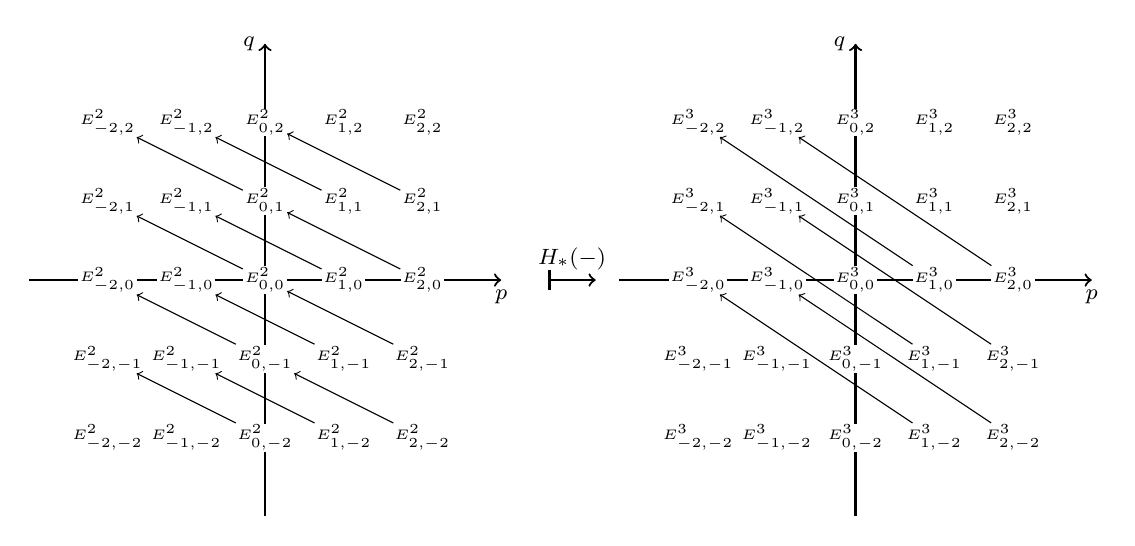
\begin{tikzpicture}[
		pagemember/.style = {
			fill = white, 
			font = \tiny, 
			inner sep = 0.5pt
		}]
		\def\xmin{-3}
		\def\xmax{3}
		\def\ymin{-3}
		\def\ymax{3}
		\begin{scope}
			\coordinate (origin) at (0, 0);
			\draw[spectral sequence/axis] (\xmin, 0) -- (\xmax, 0) node[below] {$p$};
			\draw[spectral sequence/axis] (0, \ymin) -- (0, \ymax) node[left] {$q$};
			\foreach \x [parse = true, evaluate = \x using int(\x)] in {\xmin + 1, ..., \xmax - 1}{
				\foreach \y [parse = true, evaluate = \y using int(\y)] in {\ymin + 1, ..., \ymax - 1}{
					\node[pagemember] (E2-\x-\y) at (\x, \y) {$E^2_{\x, \y}$};
				}
			}
			\foreach \x [parse = true, evaluate = \x using int(\x)] in {\xmin + 3, ..., \xmax - 1}{
				\foreach \y [parse = true, evaluate = \y using int(\y)] in {\ymin + 1, ..., \ymax - 2}{
					\tikzmath{
						int \tx, \ty;
						\tx = \x - 2;
						\ty = \y + 1;
					}
					\draw[->] (E2-\x-\y) -- (E2-\tx-\ty);
				}
			}
		\end{scope}
		\begin{scope}[xshift = 2.5 * \xmax cm]
			\coordinate (origin) at (0, 0);
			\draw[spectral sequence/axis] (\xmin, 0) -- (\xmax, 0) node[below] {$p$};
			\draw[spectral sequence/axis] (0, \ymin) -- (0, \ymax) node[left] {$q$};
			\foreach \x [parse = true, evaluate = \x using int(\x)] in {\xmin + 1, ..., \xmax - 1}{
				\foreach \y [parse = true, evaluate = \y using int(\y)] in {\ymin + 1, ..., \ymax - 1}{
					\node[pagemember] (E3-\x-\y) at (\x, \y) {$E^3_{\x, \y}$};
				}
			}
			\foreach \x [parse = true, evaluate = \x using int(\x)] in {\xmin + 4, ..., \xmax - 1}{
				\foreach \y [parse = true, evaluate = \y using int(\y)] in {\ymin + 1, ..., \ymax - 3}{
					\tikzmath{
						int \tx, \ty;
						\tx = \x - 3;
						\ty = \y + 2;
					}
					\draw[->] (E3-\x-\y) -- (E3-\tx-\ty);
				}
			}
		\end{scope}
		\draw[|->, thick] (1.2 * \xmax, 0) --++(0:.2 * \xmax) node[anchor = south, midway, font = \footnotesize] {$H_*({{-}})$};
	\end{tikzpicture}
	\caption{$E^2$- and $E^3$-pages of a homologically graded spectral sequence}
\end{figure}
\begin{definition}
	We say a spectral sequence is \strong{first quadrant}\index{spectral sequence!first quadrant} if all the groups $E^2_{p, q}$ are trivial whenever $p < 0$ or $q < 0$.
\end{definition}
\begin{figure}[ht]
	\centering
	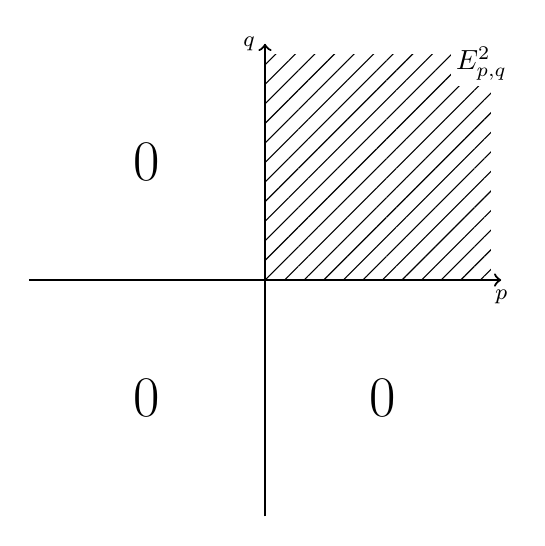
\begin{tikzpicture}[
		shaded/.style = {
			postaction = {
				pattern = {
					Lines[angle = 45, distance = 5pt]
				}
			}
		}]
		\draw[spectral sequence/axis] (-3, 0) -- (3, 0) node[below] {$p$};
		\draw[spectral sequence/axis] (0, -3) -- (0, 3) node[left] {$q$};
		\begin{scope}[anchor = center, text centered, font = \huge]
			\node at (1.5, -1.5) {$0$};
			\node at (-1.5, 1.5) {$0$};
			\node at (-1.5, -1.5) {$0$};
		\end{scope}
		\path[shaded] (0, 0) rectangle (2.87, 2.87);
		\node[draw = none, fill = white, inner sep = 2pt, outer sep = 0] at (2.75, 2.75) {$E^2_{p, q}$};
	\end{tikzpicture}
	\caption{A first-quadrant spectral sequence. All potentially nontrivial groups live in the shaded quadrant.}
\end{figure}
\begin{lemma}
	For a first quadrant spectral sequence $(E^\bullet, d^\bullet, h^\bullet)$ we have $E^r_{p, q} = 0$ if $p < 0$ or $q < 0$ for all $r \geq 2$.
	Moreover, for a given $(p, q) \in \Z \times \Z$ the map $h$ induces an isomorphism for all $r > r_0 \coloneq \max(p, q + 1)$, i.e. the groups $E^r_{p, q}$ stabilize as $r \to \infty$.
\end{lemma}
\begin{proof}
	The first statement follows immediately from the existence of $h^\bullet$ by induction on $r$.
	For the second statement, if $r > r_0$, then the target of the differential $d^r\colon E^r_{p, q} \to E^r_{p - r, q + r - 1}$ is trivial since $p - r < 0$, so every element of $E^r_{p, q}$ is a cycle.
	Moreover, the domain of the incoming differential $E^r_{p + r, q - r + 1} \to E^r_{p, q}$ is trivial since $q - r + 1 < 0$, so $E^r_{p, q} \isom H_*(E^r_{p, q}) \isom E^{r + 1}_{p, q}$.
\end{proof}
\begin{definition}
	For a first quadrant spectral sequence $(E^\bullet, d^\bullet, h^\bullet)$ we define its \strong{$E^\infty$-page}\index{$E^\infty$-page} as the bigraded abelian group
	\begin{equation*}
		E^\infty_{p, q} \coloneq E^{r_0(p, q) + 1}_{p, q}
	\end{equation*}
	with $r_0(p, q) \coloneq \max(p, q + 1)$.
	By the previous lemma, $E^\infty_{p, q} \isom E^r_{p, q}$ whenever $r > r_0(p, q)$.
\end{definition}
By a \strong{filtered object}\index{filtered object} $(H, F)$ in an abelian category $\mathcal{A}$ we mean an object $H \in \mathcal{A}$ together with a sequence of inclusions
\begin{equation*}
	0 = F^{-1} \subseteq F^0 \subseteq F^1 \subseteq \ldots \subseteq F^n \subseteq \ldots \subseteq H
\end{equation*}
We will apply this to the category of graded abelian groups and $H = H_*(E; \Z)$.
Notationally, if $(H, F)$ is a filtered object in abelian groups, we write $F^n_m$ for the $n$th object in the filtration associated to the group $H_m$; in other words, $F^0_m \subseteq F^1_m \subseteq \ldots \subseteq H_m$ is the filtration associated to $H_m$.
\begin{definition}
	A first quadrant spectral sequence is said to \strong{converge}\index{convergence!of spectral sequences} to a filtered object in graded abelian groups $(H, F)$ if there is a chosen isomorphism
	\begin{equation*}
		E^\infty_{p, q} \isom F^p_{p + q} / F^{p - 1}_{p + q}
	\end{equation*}
	for all values of $p$ and $q$ and moreover $F^p_n = H_n$ if $p \geq n$.
	In this case, we write $E^2_{p, q} \Rightarrow H$.
\end{definition}
\begin{remark}
	\leavevmode
	\begin{itemize}
		\item Convergence is really a \emph{datum} of the isomorphism $E^\infty_{p, q} \isom F^p_{p + q} / F^{p - 1}_{p + q}$ and not a property.
		\item Convergent spectral sequences are often simply encoded as $E^2_{p, q} \Rightarrow H$, but this suppresses not only this data but also the higher pages, the differentials, and the filtration on $H$!
	\end{itemize}
\end{remark}

\subsection{Fibre Sequences}
In order to be able to move onto the definition of the Serre spectral sequence for fibre sequences, let us define exactly what we mean by \enquote{fibre sequence}.
\begin{definition}
	Let $f\colon X \to Y$ be a map of spaces and $x \in X$ a point.
	The \strong{homotopy fibre}\index{homotopy fibre} $\hofib_x(f)$ of $f$ at $x$ is the space
	\begin{equation*}
		\hofib_x(f) \coloneq P_x X \times_X Y
	\end{equation*}
	where $P_x X = \{\gamma\colon I \to X \mid \gamma(1) = x\}$ is the \strong{based path space}\index{path space} of $X$.
	It comes with the evaluation at 0 map $\ev_0\colon P_x X \to X,\ \gamma \mapsto \gamma(0)$.
	In fact, it is the pullback
	\begin{equation*}
		\begin{tikzcd}
			\hofib_x(f)
					\ar[r]
					\ar[d]
					\ar[dr, phantom, "\lrcorner" very near start]
				& P_x X
					\ar[d, "\ev_0"]
			\\
			X 
					\ar[r, "f"]
				& Y
		\end{tikzcd}
	\end{equation*}
\end{definition}
In words, $\hofib_x(f)$ is the space of pairs $(\gamma, y)$ where $y \in Y$ is a points and $\gamma$ is a path from $f(y)$ to $x$.
We note that $P_x X$ is contractible via the homotopy
\begin{align*}
	H\colon P_x X \times I &\to P_x X \\
	(\gamma, t) &\mapsto (s \mapsto \gamma((1 - t)s + t))
\end{align*}
\begin{example}
	If $* \xto{f} X$ is the inclusion of any point, then $\hofib_x(f) = \Omega_x X$.
\end{example}
\begin{definition}
	A \strong{fibre sequence of topological spaces} is a sequence $F \xto{i} Y \xto{f} X$, a basepoint $x \in X$, and a homotopy $h\colon F \to X^I$ from the composite $f \circ i$ to the constant map $c_x\colon F \to X$ such that the induced map
	\begin{equation*}
		F \to \hofib_x(f),\ z \mapsto (h(z), i(z))
	\end{equation*}
	is a weak homotopy equivalence.
\end{definition}
\begin{example}\label{expl:fibresequences}
	\leavevmode
	\begin{enumerate}
		\item Let $f\colon Y \to X$ be any continuous map, $x \in X$ a point.
			Then the pair $(\hofib_x(f) \xto{i} Y \xto{f} X, h)$ where $i(\gamma, y) \coloneq y$ is a fibre sequence since by construction the map $\hofib_x(f) \to \hofib_x(f)$ is just the identity.
	\end{enumerate}
\end{example}
Every fibre sequence is equivalent to such an example in the following sense:
Given $(F \xto{i} Y \xto{f} X)$, there is a commutative diagram
\begin{equation*}
	\begin{tikzcd}
		F
				\ar[r, "\htpyeqv_w"]
				\ar[d]
			& \hofib_x(f)
				\ar[d]
		\\
		Y
				\ar[r, equal, "\id_Y"]
				\ar[d, "f"]
			& Y
				\ar[d, "f"]
		\\
		X 
				\ar[r, equal, "\id_X"]
			& X
	\end{tikzcd}
\end{equation*}
and \enquote{equivalence of fibre sequences}.
In particular, $\Omega X \to * \to X$ is a fibre sequence where $h\colon \Omega X \times I \to X$ is the evaluation map.

\strong{Warning:} If one instead chooses $h$ to be the constant homotopy, one does not obtain a fibre sequence (unless $X$ is weakly contractible) just because the induced map $\Omega X \to \hofib_x(f) = \Omega X$ is the constant map which is not a weak homotopy equivalence.
Hence, the choice of $h$ is important!

% TODO starred
\begin{example}[continuation of example \ref{expl:fibresequences}]
	\leavevmode
	\begin{enumerate}[resume]
		\item For every two spaces $F$ and $X$ and all basepoints $x \in X$, the pair $(F \to F \times X \xto{\pr_X} X, \const)$ is a fibre sequence called the \strong{trivial fibre sequence}\index{trivial fibre sequence}.
			To see this, note that
			\begin{equation*}
				\hofib_x(\pr_X) = F \times P_x X
			\end{equation*}
			with induced map $F \to F \times P_x X,\ y \mapsto (y, \const_x)$ which is a homotopy equivalence as $P_x X$ is contractible.
		\item\label{expl:fibrebundlefibresequence} Let $p\colon E \to B$ be a fibre bundle with fibre $F = p^{-1}(b)$ for some $b \in B$.
			Then the sequence $F \to E \xto{p} B$ together with the constant homotopy is a fibre sequence.
			This is a special case of the next example:
		\item Recall that $p\colon E \to B$ is a \strong{Serre fibration}\index{fibration!Serre} if in every commutative diagram of the form
			\begin{equation*}
				\begin{tikzcd}
					D^n \times \{0\}
							\ar[r]
							\ar[d, hook]
						& E
							\ar[d, "p"]
					\\
					D^n \times I
							\ar[r]
							\ar[ur, dashed]
						& B
				\end{tikzcd}
			\end{equation*}
			a lift $D^n \times I \to E$ exists making the whole diagram commute.
			Given a Serre fibration $p\colon E \to B$ and a point $b \in B$, the sequence $F = p^{-1}(b) \incl E \to B$ together with the constant homotopy is a fibre sequence (the proof of this is exercise \ref{ex:serrefib}).
		\item\label{expl:hopfbundle} As a special case of \ref{expl:fibrebundlefibresequence}, the \strong{Hopf fibration}\index{Hopf fibration} is a fibre bundle
			\begin{equation*}
				S^1 \to S^3 \xto{\eta} S^2
			\end{equation*}
			It arises by letting $S^1 = \Uni(1)$ act on $S^3 \subseteq \C^2$ via
			\begin{equation*}
				\lambda \cdot (x_1, x_2) = (\lambda x_1, \lambda x_2)
			\end{equation*}
			The quotient space of this action is $\CP^1 = S^2$.
		\item The previous example generalizes to fibre bundles
			\begin{equation*}
				S^1 \to S^{2n + 1} \to \CP^n
			\end{equation*}
			with limit case
			\begin{equation*}
				\begin{tikzcd}
					S^1
							\ar[r]
							\ar[d, "\htpyeqv"]
						& S^\infty
							\ar[r]
							\ar[d, "\htpyeqv"]
						& \CP^\infty
							\ar[d, equal]
					\\
					\Omega \CP^\infty
							\ar[r]
						& * 
							\ar[r]
						& \CP^\infty
				\end{tikzcd}
			\end{equation*}
	\end{enumerate}
\end{example}

\subsection{The Serre Spectral Sequence}\lecture{16.10.23}
We are now ready to show the existence of the Serre spectral sequence:
\begin{theorem}[Serre]\index{Serre spectral sequence}
	For every fibre sequence $(F \to Y \to X, h)$ with $X$ simply connected and abelian group $A$ there exists a first quadrant spectral sequence of the form
	\begin{equation}\label{s3:defn}
		E^2_{p, q} = H_p(X; H_q(F; A)) \Rightarrow H_{p + q}(Y; A)
	\end{equation}
\end{theorem}
The expression in \ref{s3:defn} does not include information about the differentials and higher pages, nor about the filtration on $H_*(Y; A)$ and the identification of its subquotients with the $E^\infty$-page.

% TODO understand this
One edge case is easy to state:
The map
\begin{equation*}
	H_n(F; A) \isom H_0(Y; H_n(F; A)) = E^2_{0, n} \twoheadrightarrow E^\infty_{0, n} \incl H_n(Y; A)
\end{equation*}
agrees with the factorization
\begin{equation*}
	\begin{tikzcd}
		H_n(X; A) 
				\ar[r, two heads]
				\ar[rr, bend right, swap, "H_n(c; A)"]
			& \img
				\ar[r, hook]
			& H_n(Y; A)
	\end{tikzcd}
\end{equation*}

Before proving the theorem, let us first look at some examples.
\begin{example}\index{Hopf fibration}
	We revisit the Hopf fibration
	\begin{equation*}
		S^1 \incl S^3 \xto{\eta} S^2
	\end{equation*}
	The $E^2$-page of its Serre spectral sequence looks like this:
	\begin{equation*}
		\begin{tikzpicture}[
			pagemember/.style = {
				fill = white, 
				font = \scriptsize, 
				inner sep = 0.5pt
			},
			big zero/.style = {
				anchor = center,
				text centered,
				font = \Large
			}]
			\matrix[
				matrix of math nodes, 
				name = m, 
				nodes in empty cells, 
				nodes = {outer sep = 0ex},
				column sep = {4ex, between origins},
				row sep = 0.5ex,
				column 1/.style = {anchor = base east, font = \scriptsize}, 
				row 3/.style = {font = \scriptsize}] {
					1 &[-1.9ex] A & 0 & A \\
					0 & A & 0 & A \\
					& 0 & 1 & 2 \\
			};
			\draw[spectral sequence/axis] (m-2-2.south west) -- (m-1-2.north west) -- ++(0, 1.5) node[left] (q) {$q$};
			\draw[spectral sequence/axis] (m-2-2.south west) -- (m-2-4.south east) -- ++(1.5, 0) node[below] (p) {$p$};
			% need to compute a bunch of helper coordinates to position the big 0s
			\coordinate (a) at ($(m-1-2.north west)!.5!(q)$); % roughly the midpoint of part of the y-axis "above" the matrix
			\coordinate (b) at (m-1-3 |- a); % point at that midpoint's height centered above the "middle" top row matrix entry
			\node[big zero] (leftzero) at (b) {$0$};

			\coordinate (c) at ($(m-1-4.center)!.5!(m-2-4.center)$); % midpoint between the first two matrix entries in the rightmost column
			\coordinate (d) at ($(m-2-4.south east)!.5!(p)$); % rough midpoint of the x-axis segment "after" the matrix raised
			\coordinate (e) at (d |- c); % d raised to the height of c
			\node[big zero] (rightzero) at (e) {$0$};

			\node[big zero] (toprightzero) at (rightzero |- leftzero) {$0$};

			\coordinate (topright) at (p |- q); % the very top right
			\node[draw, fill = white, inner sep = 2pt, outer sep = 0, font = \footnotesize] at ($(topright) + (-0.15, -0.15)$) {$E^2_{p, q}$}; % label

			\draw[commutative diagrams/every arrow, thick, preaction = {draw = white, arrows = -, line width = 0.5ex}] (m-2-4) -- (m-1-2); % differential
		\end{tikzpicture}
	\end{equation*}
	There is only one potentially non-trivial $d^2$-differential, namely
	\begin{equation*}
		d^2\colon E^2_{2, 0} \to E^2_{0, 1}
	\end{equation*}
	All higher differentials are necessarily trivial for degree reasons.
	Hence, the $E^\infty$-page looks as follows:
	\begin{equation*}
		\begin{tikzpicture} [
			pagemember/.style = {
				fill = white, 
				font = \scriptsize, 
				inner sep = 0.5pt
			},
			big zero/.style = {
				anchor = center,
				text centered,
				font = \Large
			}]
			\matrix[
				matrix of math nodes, 
				name = m, 
				nodes in empty cells, 
				nodes = {outer sep = 0ex},
				column sep = {5.5ex, between origins},
				row sep = 0.5ex,
				font = \footnotesize,
				column 1/.style = {anchor = base east, font = \scriptsize}, 
				row 3/.style = {font = \scriptsize}] {
					1 &[-1.9ex] \coker d^2 & 0 & A \\
					0 & A & 0 & \ker d^2 \\
					& 0 & 1 & 2 \\
			};
			\coordinate (help1) at (m-1-2.west |- m-2-2.south west);
			\draw[spectral sequence/axis] (help1) -- (m-1-2.north west) -- ++(0, 1.5) node[left] (q) {$q$};
			\draw[spectral sequence/axis] (help1) -- (m-2-4.south east) -- ++(1.5, 0) node[below] (p) {$p$};
			% need to compute a bunch of helper coordinates to position the big 0s
			\coordinate (a) at ($(m-1-2.north west)!.5!(q)$); % roughly the midpoint of part of the y-axis "above" the matrix
			\coordinate (b) at (m-1-3 |- a); % point at that midpoint's height centered above the "middle" top row matrix entry
			\node[big zero] (leftzero) at (b) {$0$};

			\coordinate (c) at ($(m-1-4.center)!.5!(m-2-4.center)$); % midpoint between the first two matrix entries in the rightmost column
			\coordinate (d) at ($(m-2-4.south east)!.5!(p)$); % rough midpoint of the x-axis segment "after" the matrix raised
			\coordinate (e) at (d |- c); % d raised to the height of c
			\node[big zero] (rightzero) at (e) {$0$};

			\node[big zero] (toprightzero) at (rightzero |- leftzero) {$0$};

			\coordinate (topright) at (p |- q); % the very top right
			\node[draw, fill = white, inner sep = 2pt, outer sep = 0, font = \footnotesize] at ($(topright) + (-0.15, -0.15)$) {$E^\infty_{p, q}$}; % label
		\end{tikzpicture}
	\end{equation*}
	We know that $H_n(S^3; A) \isom A$ if $n = 0, 3$ and 0 else, so from the $E^\infty$-page we obtain that $H_0(S^3; A) \isom A$, $H_1(S^3; A) \isom \coker d^2$, $H_2(S^3; A) \isom \ker d^2$, and $H_3(S^3; A) \isom A$. 
	Thus, $d^2\colon E^2_{2, 0} \to E^2_{0, 1}$ must be an isomorphism.
\end{example}
\begin{figure}[ht]
	\centering
	\caption{The $E^2$-page $E^2_{p, q} = H_p(S^2; H_q(S^1; A))$ of the Serre spectral sequence for the Hopf fibration $S^1 \incl S^3 \xto{\eta} S^2$.}
	\label{fig:hopffibhomspecseq}
\end{figure}

\begin{lemma}
	There is a fibre bundle
	\begin{equation*}
		\Uni(n - 1) \xto{i} \Uni(n) \to S^{2n - 1}
	\end{equation*}
	where $\Uni(n)$ denotes the topological group of unitary $(n \times n)$-matrices and $i$ is the standard inclusion which adds a trivial $\C$-summand:
	\begin{equation*}
		i(A) = \begin{pmatrix}
			A & 0 \\
			0 & 1
		\end{pmatrix}
	\end{equation*}
\end{lemma}
\begin{proof}
	The group $\Uni(n)$ acts on $\C^n$ by definition.
	This action restricts to the unit sphere $S^{2n - 1} \subseteq \C^n$.
	Furthermore, this action is transitive because every length 1 vector can be extended to an orthonormal basis.
	Hence, $S^{2n - 1}$ is in bijection with the \enquote{orbit space} $\Uni(n) / \Stab(x)$ for any $x \in S^{2n - 1}$ where $\Stab(x) \coloneq \{A \in \Uni(n) \mid Ax = x\}$ is the \emph{stabilizer} of $x$.
	For $x = (0, \ldots, 0, 1)$, this stabilizer equals $\Uni(n - 1)$.
	We obtain a continuous bijection
	\begin{align*}
		\Uni(n) / \Uni(n - 1) &\to S^{2n - 1} \\
		A \cdot \Uni(n - 1) &\mapsto A \cdot (0, \ldots, 0, 1)
	\end{align*}
	As $\Uni(n) / \Uni(n - 1)$ is quasi-compact and $S^{2n - 1}$ is Hausdorff, this map is a homeomorphism.
	% TODO: cite Lee
	Finally, we use the fact that for a smooth free action of a compact Lie group $G$ on a manifold $M$, the map $M \to M / G$ is always a fibre bundle (in fact a $G$-principal bundle).
\end{proof}
\begin{example}
	We consider the case $n = 2$, i.e. the fibre sequence $S^1 \isom \Uni(1) \to \Uni(2) \to S^3$.
	Our goal is to compute the homology of $\Uni(2)$ via the Serre spectral sequence.
	All differentials on all pages have to be trivial for degree reasons.
	Hence the $E^\infty$-page equals the $E^2$-page.
	Moreover, every antidiagonal has at most one non-trivial term, so we can read off
	\begin{equation*}
		H_n(\Uni(2); \Z) \isom \begin{cases}
			\Z & n = 0, 1, 3, 4 \\
			0  & \text{else}
		\end{cases}
	\end{equation*}
	In fact, one can show that $\Uni(2)$ is in fact homeomorphic to $S^3 \times \Uni(1)$, so this statement could also be derived from the Künneth theorem.
\end{example}
\begin{example}
	Next, we consider the fibre sequence $\Uni(2) \to \Uni(3) \to S^5$.
	The first potentially non-trivial differential is a $d^5$, the map
	\begin{equation*}
		d^5\colon \underbrace{E^5_{5, 0}}_{\isom \Z} \to \underbrace{E^5_{0, 4}}_{\isom \Z}
	\end{equation*}
	At this point, we cannot decide what the differential is (at least not without resorting to tools like Poincaré duality).
	All higher differentials are again trivial for degree reasons and all filtrations collapse to at most one entry, so we obtain
	\begin{equation*}
		H_n(\Uni(3); \Z) \isom \begin{cases}
			\Z 			& n = 0, 1, 3, 6, 8, 9 \\
			\coker d^5 	& n = 4 \\
			\ker d^5 	& n = 5 \\
			0 			& \text{else}
		\end{cases}
	\end{equation*}
	This example illustrates a typical situation, namely that one can often not fully determine all differentials but still deduce a lot of information.
	We will soon see that $d^5 = 0$ and hence $H_4(\Uni(3); \Z) \isom H_5(\Uni(3); \Z) \isom \Z$.
\end{example}
\begin{example}
	We consider $\Uni(3) \to \Uni(4) \to S^7$.
	The only possible non-trivial differentials are
	\begin{align*}
		d^7\colon E^7_{7, 0} &\to E^7_{0, 6} \\
		d^7\colon E^7_{7, 5} &\to E^7_{0, 9}
	\end{align*}
	which we cannot compute at this point.
	Nevertheless we can still deduce a lot, for example that
	\begin{equation*}
		H_n(\Uni(4); \Z) \isom \begin{cases}
			\Z 					& n = 0, 1, 3 \\
			H_4(\Uni(3); \Z) 	& n = 4 \\
			H_5(\Uni(3); \Z) 	& n = 5 \\
			0 					& n = 2
		\end{cases}
	\end{equation*}
	and that there is a short exact sequence
	\begin{equation*}
		0 \to \Z \to H_8(\Uni(4); \Z) \to \Z \to 0
	\end{equation*}
	which splits to yield $H_8(\Uni(4); \Z) \isom \Z \dsum \Z$.
\end{example}

In the previous examples we used the Serre spectral sequence to compute the homology of the total space of the fibre sequence.
We now show that it can be used to compute the homology of the basespace or fibre.
\begin{example}
	We consider the fibre sequence $S^1 \to S^{2n + 1} \to \CP^n$ for $n \geq 2$.
	Let us pretend that we do not know $H_*(\CP^n)$.
	Since $H_1(S^{2n + 1}; \Z) = 0$, there must be a surjective $d^2$-differential $d^2\colon E^2_{2, 0} \to E^2_{0, 1}$.
	As $H_2(S^{2n + 1}; \Z) = 0$, this differential must be injective, so $\Z \isom E^2_{2, 0} = H_2(\CP^n; H_0(S^1; \Z)) = H_2(\CP^n; \Z)$.
	Furthermore, we see that $H_1(\CP^n; \Z) = E^2_{1, 0} = 0$.
	This implies that $E^2_{1, 1} = H_1(\CP^n; H_1(S^1; \Z)) = 0$ and $E^2_{2, 1} = H_2(\CP^n; H_1(S^1; \Z)) \isom \Z$ as $H_1(S^1; \Z) \isom \Z$.
	Since we also have $H_3(S^{2n + 1}; \Z) = 0$, we can repeat the same argument to deduce that $d^2\colon E^2_{4, 0} = H_4(\CP^n; H_0(S^1; \Z)) \to E^2_{2, 2} \isom \Z$ must be an isomorphism, hence $H_4(\CP^n; \Z) \isom \Z$.
	This can be iterated until we get the following picture: % TODO
	Since $H_{2n + 1}(S^{2n + 1}; \Z) \isom \Z$, we cannot conclude that the $\Z$ in bidegree $(2n, 1)$ must be the image of a differential.
	There are then two possibilities:
	\begin{enumerate}
		\item $d^2\colon E^2_{2n + 2, 0} \to E^2_{2n, 1}$ is trivial.
			This implies $E^2_{2n + 2, 0} = 0$ and by induction that $E^2_{p, q} = 0$ for all $p > 2n$; or
		\item $d^2\colon E^2_{2n + 2, 0} \to E^2_{2n, 1} \isom \Z$ is non-zero.
			Since its cokernel is isomorphic to the lowest term of the filtration on $H_{2n + 1}(S^{2n + 1}; \Z) \isom \Z$, this forces $d^2$ to be surjective as no $\Zn{n}$ with $n > 1$ embeds into $\Z$.
			We obtain the following pattern: % TODO
			This can be ruled out using e.g. that $\CP^n$ is $2n$-dimensional CW-complex and therefore $H_k(\CP^n; \Z) = 0$ for $k > 2n$.
	\end{enumerate}
	We thus obtain 
	\begin{equation*}
		H_k(\CP^n; \Z) \isom \begin{cases}
			\Z & k = 2, 4, \ldots, 2n \\
			0  & \text{else}
		\end{cases}
	\end{equation*}
\end{example}

\lecture{20.10.23}
Next, we turn to an exercise of how the Serre spectral sequence can be used to compute the homology of the fibre.
\begin{example}
	We consider the fibre sequence
	\begin{equation*}
		\Omega S^3 \to * \to S^3
	\end{equation*}
	The $E^2$-page looks like this:
	The homotopy of the point trivial in positive degree, so we must have $E^\infty_{p, q} = 0$ unless $p = q = 0$.
	The only non-trivial differentials are $d^3$s, so we conclude that $d^3\colon E^3_{3, q} \to E^3_{0, q + 2}$ must be an isomorphism for all $q \in \N$.
	As $E^3_{3, q} \isom H_3(S^3; H_q(\Omega S^3; \Z)) \isom H_q(\Omega S^3; \Z)$ and $E^3_{0, q + 2} \isom H_0(S^3; H_{q + 2}(\Omega S^3; \Z)) \isom H_{q + 2}(\Omega S^3; \Z)$ and finally $H_0(\Omega S^3; \Z) \isom \Z$, this implies that $H_k(\Omega S^3; \Z) \isom \Z$ if $k$ is even and 0 else, and the $E^3$-page looks like this:
	In particular, we see that $\Omega S^3$ is infinite-dimensional.
\end{example}

We now discuss the cohomological version of the Serre spectral sequence and its multiplicative structure.
The multiplication also helps in determining the differentials, for example for the spectral sequences computing (co)homology of unitary groups.
\begin{definition}
	A \strong{cohomologically-graded spectral sequence}\index{spectral sequence!cohomologically graded}	is a triple $(E_\bullet, d_\bullet, h_\bullet)$ where
	\begin{itemize}
		\item $(E_r)_{r \geq 2}$ is a sequence of bigraded abelian groups,
		\item $d_r\colon E_r \to E_r$ is a sequence of differentials (satisfying $d_r^2 = 0$) of bidegree $(r, 1 - r)$, and
		\item $h_r\colon H_*(E_r) \to E_{r + 1}$ is a sequence of bigrading-preserving isomorphisms.
	\end{itemize}
\end{definition}
As before we define what it means for a spectral sequence to be \strong{first quadrant}\index{spectral sequence!first quadrant} (namely $E^{p, q}_2 = 0$ if $p < 0$ or $q < 0$) and the \strong{$E^\infty$-page}\index{$E^\infty$-page}.
For convergence, we consider descending filtrations $H = F_0 \supseteq F_1 \supseteq \cdots$ instead of the ascending filtrations $0 = F^{-1} \subseteq F_0 \subseteq \cdots \subseteq H$ used in the homologically graded case.
\begin{definition}
	A cohomological first quadrant spectral sequence is said to \strong{converge}\index{convergence!of spectral sequences} to a filtered object $(H, F)$ in graded abelian groups if there are isomorphisms $E^{p, q}_\infty \isom F^{p + q}_p / F^{p + q}_{p + 1}$ for all $p, q$ and if $F^n_p = 0$ if $p \geq n$.
	As before, we write $E^{p, q}_2 \Rightarrow H$.
\end{definition}
\begin{definition}
	A (\strong{commutative}) \strong{multiplicative structure}\index{multiplicative structure!on a spectral sequence} on a cohomologically graded spectral sequence $(E_\bullet, d_\bullet, h_\bullet)$ is a bigraded (commutative) ring structure on $E_\bullet$, i.e. associative multiplication maps
	\begin{equation*}
		E_r^{p, q} \tensor E_r^{p', q'} \to E_r^{p + p', q + q'}
	\end{equation*}
	such that $d_r\colon E_r \to E_r$ is a \emph{graded derivation}\index{graded derivation}, that is to say
	\begin{equation*}
		d_r(x \cdot y) = d_r(x) \cdot y + (-1)^{p + q} x \cdot d_r(y)
	\end{equation*}
	for all $x$ in bidegree $(p, q)$ and all $y$.
	Commutativity here is meant in the graded sense: $x \cdot y$ = $(-1)^{(p + q)(p' + q')} y \cdot x$.

	As a result, each $H_*(E_r)$ is a bigraded ring and we accordingly require the maps $h_\bullet\colon H_*(E_\bullet) \xto{\isom} E_{\bullet + 1}$ to be isomorphisms of bigraded rings.
	Furthermore, the $E_\infty$-page also inherits the structure of a (commutative) bigraded ring.
\end{definition}
\begin{definition}\index{multiplicative filtration}
	A filtration $\cdots \subseteq F_n \subseteq \cdots \subseteq F_1 \subseteq F_0 = H$ on a graded ring $H$ is said to be \strong{multiplicative} or \strong{compatible with the multiplicative structure} if $F_s \cdot F_t \subseteq F_{s + t}$.
	We say that $(H, F)$ is a \strong{filtered graded ring}\index{filtered graded ring}.
\end{definition}
It follows that the associated graded group $\bigdsum_p F_p / F_{p + 1}$ of a filtered graded (commutative) ring is a bigraded (commutative) ring.

\begin{definition}
	A multiplicative first quadrant spectral sequence $(E_\bullet, d_\bullet, h_\bullet)$ is said to \strong{converge}\index{convergence!of spectral sequences} to a filtered graded ring $(H, F)$ if it converges additively and the chosen isomorphisms $E_\infty^{p, q} \isom F^{p + q}_p / F^{p + q}_{p + 1}$ is compatible with the graded ring structure.
\end{definition}
\begin{theorem}[Serre]\index{Serre spectral sequence}
	For every fibre sequence of spaces $(F \to Y \to X, h)$ with simply connected base space $X$ and every abelian group $A$ there exists a first quadrant spectral sequence of the form
	\begin{equation*}
		E^{p, q}_2 = H^p(X; H^q(F; A)) \Rightarrow H^{p + q}(Y; A)
	\end{equation*}
	If $A = R$ is a (commutative) ring, then the spectral sequence and its convergence are multiplicative where on the $E_2$-page the multiplication is given by $(-1)^{q \cdot p'}$ times the composite 
	\begin{equation*}
		\begin{tikzcd}
			H^p(X; H^q(F; R)) \tensor_R H^{p'}(X; H^{q'}(F; R))
					\ar[d]
			\\
			H^{p + p'}(X; H^q(F; R) \tensor_R H^{q'}(F; R))
					\ar[d]
			\\
			H^{p + p'}(X; H^{q + q'}(F; R))
		\end{tikzcd}
	\end{equation*}
\end{theorem}
\begin{note}
	If $H^*(F; R)$ or $H^*(X; R)$ is flat (e.g. free) and of finite type over $R$, then the $E_2$-page is isomorphic to the graded tensor product of $H^*(X; R)$ and $H^*(F; R)$.
\end{note}
\begin{example}
	We reconsider the fibre sequence
	\begin{equation*}
		\Uni(1) \to \Uni(2) \to S^3
	\end{equation*}
	There can be no non-trivial differentials.
	As a graded ring, the $E_2$-page and thus also the $E_\infty$-page are isomorphic to $H^*(S^3; \Z) \tensor_{\Z} H^*(\Uni(1); \Z)$.
	Let $x_1 \in H^1(\Uni(1); \Z)$ and $x_3 \in H^3(S^3; \Z)$ be generators.
	Then $H^*(\Uni(1); \Z) \isom \Lambda(x_1)$ and $H^*(S^3; \Z) \isom \Lambda(x_3)$ where $\Lambda(M)$ denotes the \emph{exterior algebra}\index{exterior algebra} on a set $M$, i.e. the free algebra on $M$ modulo the relations $x_i x_j = -x_j x_i$ and $x_i^2 = 0$ for all $x_i, x_j \in M$.
	Hence, the $E_2$-page is the exterior algebra $\Lambda(x_1, x_3)$ and the $\Z$ in bidegree $(3, 1)$ is spanned by $x_1 x_3$.
	The filtration collapses degree-wise and hence $H^*(\Uni(2); \Z)$ is exterior on classes $x_1 \in H^1(\Uni(2); \Z)$ and $x_3 \in H^3(\Uni(2); \Z)$ that are uniquely determined by the spectral sequence.
\end{example}
\begin{example}
	We move on to the fibre sequence $\Uni(2) \to \Uni(3) \to S^5$.
	Again, the $E_2$-page is given by $H^*(S^5; \Z) \tensor_{\Z} H^*(\Uni(2); \Z) \isom \Lambda(x_1, x_3, x_5)$ where $x_5 \in H^5(S^5; \Z)$ is a generator.
	There is only one possibly non-trivial differential $d_5\colon E_5^{0, 4} \to E_5^{5, 0}$.
	However, the product rule implies 
	\begin{equation*}
		d_5(x_1 x_3) = \underbrace{d_5(x_1)}_{= 0} \cdot x_3 + (-1)^{1 + 0} x_1 \cdot \underbrace{d_5(x_3)}_{= 0} = 0
	\end{equation*}
	Again the filtration collapses and hence $H^*(\Uni(3); \Z) \isom \Lambda(x_1, x_3, x_5)$.
\end{example}
\begin{example}
	We revisit $\Uni(3) \to \Uni(4) \to S^7$.
	As before, the product rule implies that all $d_7$-differentials must be trivial.
	There is a non-trivial filtration on $H^8(\Uni(4); \Z)$ of the form
	\begin{equation*}
		0 \to \underbrace{E_\infty^{7, 1}}_{\substack{\isom \Z[x_1 x_7] \\ \isom \Z}} \to H^8(\Uni(4); \Z) \to \underbrace{E_\infty^{0, 8}}_{\substack{\isom \Z[x_3 x_5] \\ \isom \Z}} \to 0
	\end{equation*}
	Additively, this sequence splits, but one has to be careful with the multiplicative structure.
	To resolve this, we are precise with the differentiation between the classes $x_1, x_3, x_5, x_7$ on the $E_\infty$-page and the corresponding classes $\bar{x}_1, \bar{x}_3, \bar{x}_5, \bar{x}_7 \in H^*(\Uni(4); \Z)$.
	Note that the choice of each $\bar{x}_i$ is unique since the filtration collapses in degrees 0 to 7.
	Furthermore, we record their filtrations: $\bar{x}_1$ is in $F^1_0$, $\bar{x}_3$ is in $F^3_0$, $\bar{x}_5$ is in $F^5_0$, and $\bar{x}_7$ is in $F^7_7$.
	It follows that $\bar{x}_1 \cdot \bar{x}_7$ is a generator of $F^8_7$ and that $\bar{x}_3 \cdot \bar{x}_5$ maps to a generator of $F^8_0 / F^8_1$.
	Hence $H^8(\Uni(4); \Z)$ is a free group on $\bar{x}_1 \cdot \bar{x}_7$ and $\bar{x}_3 \cdot \bar{x}_5$, and it follows that $H^*(\Uni(4); \Z) \isom \Lambda(\bar{x}_1, \bar{x}_3, \bar{x}_5, \bar{x}_7)$.
\end{example}
\begin{theorem}
	For all $n \in \N$ there is an isomorphism of graded rings
	\begin{equation*}
		H^*(\Uni(n); \Z) \isom \Lambda(x_1, \ldots, x_{2n - 1})
	\end{equation*}
	where each $x_i$ has degree $i$.
\end{theorem}
\lecture{23.10.23}
\begin{proof}
	We will do an induction on $n$.
	The case $n = 1$ is clear.
	Let thus $n \geq 2$ and assume that the statement is true for $n - 1$.
	Consider the Serre spectral sequence for the fibre sequence
	\begin{equation*}
		\Uni(n - 1) \to \Uni(n) \to S^{2n - 1}
	\end{equation*}
	By induction, its $E_2$-page is isomorphic to $H^*(S^{2n - 1}; \Z) \tensor H^*(\Uni(n - 1); \Z) \isom \Lambda(x_{2n - 1}) \tensor \Lambda(x_1, x_3, \ldots, x_{2n - 3})$ with $|x_{2n - 1}| = (2n - 1, 0)$ and $|x_i| = (0, i)$ for all $i = 1, 3, \ldots, 2n - 3$.
	For degree reasons, $d_{2n - 1}$ vanishes on all generators $x_1, x_3, \ldots, x_{2n - 3}, x_{2n - 1}$.
	By the product rule, $d_{2n - 1}$ vanishes on all elements.
	Hence, the $E_\infty$-page is isomorphic to the $E_2$-page and therefore an exterior algebra on $\Lambda(x_1, x_3, \ldots, x_{2n - 1})$.
	The filtrations on $H^*(\Uni(n); \Z)$ collapse in degrees $0, \ldots, 2n - 2$, hence we obtain unique lifts $\bar{x}_1, \ldots, \bar{x}_{2n - 1} \in H^*(\Uni(n); \Z)$.
	We only know that $x_i^2$ is of lower filtration from the spectral sequence and hence a multiple of $\bar{x}_{2n - 1}$, but not necessarily that $\bar{x}_i^2 = 0$.
	However, we know from the additive structure (all the subquotients are free over $\Z$) that $H^*(\Uni(n); \Z)$ is torsion-free as the multiplication is graded-commutative.
	We hence have $\bar{x}_i^2 = 0$.
	Thus, we obtain a ring map
	\begin{equation*}
		f\colon \Lambda(\bar{x}_1, \bar{x}_3, \ldots, \bar{x}_{2n - 1}) \to H^*(\Uni(n); \Z)
	\end{equation*}
	by sending $\bar{x}_i \to \bar{x}_i$.
	We define a grading on $\Lambda(\bar{x}_1, \bar{x}_3, \ldots, \bar{x}_{2n - 1})$ by setting the degree of $\bar{x}_1, \ldots, \bar{x}_{2n - 3}$ to be 0 and the degree of $\bar{x}_{2n - 1}$ to be $2n - 1$.
	This induces a filtration by setting $F_i$ to be the direct sum of the graded pieces of degree $\geq i$. 
	Then $f$ is filtration-preserving and induces an isomorphism on associated graded pieces.
	We now use:
	\begin{lemma}
		Let $A, B$ be graded abelian groups equipped with filtrations
		\begin{gather*}
			\cdots \subseteq F_2 \subseteq F_1 \subseteq F_0 \subseteq A \\
			\cdots \subseteq G_2 \subseteq G_1 \subseteq G_0 \subseteq B
		\end{gather*}
		which are in every degree eventually 0.
		If we have a graded filtration-preserving morphism $f\colon A \to B$ that induces an isomorphism on all associated graded pieces
		\begin{equation*}
			F_i / F_{i + 1} \xto{\isom} G_i / G_{i + 1}
		\end{equation*}
		then it is an isomorphism.
	\end{lemma}
	\begin{smallproof}
		This is an iterated \enquote{5-lemma} argument.
	\end{smallproof}
	This finishes the proof
\end{proof}
\begin{example}
	We revisit the fibre sequence
	\begin{equation*}
		S^1 \to S^{2n + 1} \to \CP^n
	\end{equation*}
	and use the Serre spectral sequence to compute the ring $H^*(\CP^n; \Z)$.
	Arguing analogously to the homological case, the $E_2$-page looks as follows:
	Let $e$ be a generator for $E_2^{0, 1}$.
	Then $x \coloneq d_2(e)$ is a generator for $E_2^{2, 0}$ and $e x$ is a generator for $E_2^{2, 1}$.
	Hence, $d_2(ex)$ generates $E_2^{4, 0}$.
	By the product rule, we have
	\begin{equation*}
		d_2(ex) = \underbrace{d_2(e)}_{= x} \cdot x + (-1)^1 e \cdots \underbrace{d_2(x)}_{= 0} = x^2
	\end{equation*}
	Hence $x^2$ generates $E_2^{4, 0} \isom H^4(\CP^n; \Z)$.
	Similarly, $d_2(ex^2)$ generates $E_2^{6, 0}$ and
	\begin{equation*}
		d_2(ex^2) = \underbrace{d_2(e)}_{= x} \cdot x^2 - e \cdot \underbrace{d_2(x^2)}_{0} = x^3
	\end{equation*}
	We obtain an isomorphism $H^*(\CP^n; \Z) \isom \Z[x] / (x^{n + 1})$ and in the limit $H^*(\CP^\infty; \Z) \isom \Z[x]$.
\end{example}
\begin{example}
	Next we compute the ring structure on $H^*(\Omega S^3; \Z)$.
	Dual to before, we obtain the following $E_2$-page:
	Let $x \in H^2(\Omega S^3; \Z) \isom E_3^{0, 2}$ be a generator.
	Then $e \coloneq d_3(x)$ generates $E_3^{3, 0}$ and $ex$ generates $E_3^{3, 2}$.
	We have 
	\begin{equation*}
		d_3(x^2) = d_3(x) \cdot x + (-1)^2 x \cdot d_3(x) = d_3(x) \cdot x + x \cdot d_3(x) = 2ex
	\end{equation*}
	Hence $x^2$ is twice a generator of $H^4(\Omega S^3; \Z)$, which we denote by \enquote{$x^2 / 2$}.
	Similarly, we find that
	\begin{equation*}
		d_3(x^3) = d_3(x) \cdot x^2 + x d_3(x^2) = ex^2 + 2ex^2 = 3ex^2 = 6 \underbrace{6 e (x^2 / 2)}_{\text{generator of } E_3^{3, 4}}
	\end{equation*}
	Inductively, we get that $x^n$ is $n!$ times a generator of $H^{2n}(\Omega S^3; \Z)$.
	We get an isomorphism
	\begin{align*}
		H^*(\Omega S^3; \Z) &\isom \Z\bigg[x, \frac{x^2}{2!}, \frac{x^3}{3!}, \ldots\bigg] \subseteq \Q[x] \\
							&\isom \Z[x_1, x_2, \ldots] / \langle \binom{n + m}{n} x_{m + n} = x_m x_n \rangle \\
							&\eqcolon \Gamma(x)
	\end{align*}
	We call $\Gamma(x)$ a \strong{divided power algebra}\index{divided power algebra} on one generator.
	Note that $\Gamma(x)$ is not finitely generated as a ring (and therefore not isomorphic to $\Z[x]$)!
\end{example}
\begin{remark}
	There is also a ring structure on the \emph{homology} $H_*(\Omega S^3; \Z)$ induced by the H-space (in fact $A_\infty$- or $E_1$-space) structure via concatenation of loops.
	One can show that $H_*(\Omega S^3; \Z)$ is actually a polynomial ring on one generator in degree 2.
	More generally, if $H_*(X; \Z)$ is free over $\Z$ then $H_*(\Omega \Sigma X; \Z)$ is the tensor algebra on $H_*(X; \Z)$ (this is the \strong{Bott-Samelson theorem}\index{Bott-Samelson theorem}) and the map
	\begin{equation*}
		H_*(X; \Z) \to H_*(\Omega \Sigma X; \Z) \isom \Tang(H_*(X; \Z))
	\end{equation*} 
	is induced by the map $X \to \Omega \Sigma X$.
\end{remark}
\begin{remark}
	Let us compare $\Omega S^3$ and $\CP^\infty$:
	Both spaces have isomorphic homology groups and a CW-structure with exactly one cell in each dimension.
	However, they have very different homotopy groups: $\pi_n \CP^\infty = 0$ for $n > 2$ whereas $\pi_n \Omega S^3 \isom \pi_{n + 1} S^3 \neq 0$ for all $n \geq 2$ (although this is a rather difficult theorem).
	They also have non-isomorphic cohomology rings as we just showed: $H^*(\CP^\infty; \Z) \isom \Z[x]$ whereas $H^*(\Omega S^3; \Z) \isom \Gamma(x)$.
	Comparing the attaching maps $S^3 \to S^2$ of the 4-cell, we know that for $\CP^\infty$ it is a generator of $\pi_3 S^2$ while for $\Omega S^3$ it is twice a generator (this follows from the fact that $x^2 \in H^4(\Omega S^3; \Z)$ is twice a generator (via the Hopf invariant)).
	Finally, both are loopspaces (as $\CP^\infty \htpyeqv \Omega K(\Z, 3)$) but $H_*(\Omega S^3; \Z)$ is polynomial while $H_*(\CP^\infty; \Z)$ is a divided power algebra.
\end{remark}
\begin{example}
	We consider the map
	\begin{equation*}
		S^3 \to K(\Z, 3)
	\end{equation*}
	classifying a generator of $H^3(S^3; \Z) \isom \Z$ (equivalently, inducing an iso on $\pi_3({{-}})$).
	Let $X$ denote the homotopy fibre of this map so that 
	\begin{equation*}
		X \to S^3 \to K(\Z, 3)
	\end{equation*}
	is a fibre sequence.
	By the long exact sequence in homotopy, $X$ is 3-connected and $\pi_n X \xto{\isom} \pi_3 S^3$ for $n \geq 4$. 
	We want to understand the (co)homology of $X$.
	As we do not know $H_*(K(\Z, 3); \Z)$ yet, we take a second homotopy fibre yielding a fibre sequence
	\begin{equation*}
		\underbrace{\Omega K(\Z, 3)}_{\htpyeqv \CP^\infty} \to X \to S^3
	\end{equation*}
	We obtain the following Serre spectral sequence:
	Since $X$ is 3-connected, $d_3\colon E_3^{0, 2} \to E_3^{3, 0}$ must be an isomorphism.
	Let $x \in E_2^{0, 2}$ be a generator.
	By the product rule,
	\begin{equation*}
		d_3(x^2) = d_3(x) x + x d_3(x) = 2 d_3(x)x
	\end{equation*}
	is twice a generator.
	Inductively, $d_3(x^n)$ is $n$ times a generator of $E_2^{3, 2n - 2}$ and hence
	\begin{equation*}
		\tilde{H}^n(X; \Z) \isom \begin{cases}
			\Zn{k}  & n = 2k + 1 \\
			0 		& \text{else}
		\end{cases}
	\end{equation*}
	with trivial cup product.
	By the universal coefficient theorem, we get
	\begin{equation*}
		\tilde{H}_n(X; \Z) \isom \begin{cases}
			\Zn{k} 	& n = 2k \\
			0 	  	& \text{else}
		\end{cases}
	\end{equation*}
\end{example}
\begin{corollary}
	We have $\pi_4 S^3 \isom \Zn{2}$ and $\pi_4 S^2 \isom \Zn{2}$ as well.
\end{corollary}
\begin{proof}
	$X$ is 3-connected and $H_4(X; \Z) \isom \Zn{2}$.
	The Hurewicz theorem then says that $\pi_4 X \isom \Zn{2}$.
	Furthermore we saw that $\pi_n X \xto{\isom} S^3$ for $n \geq 4$.
	Finally, by the Hopf fibration $S^1 \to S^3 \to S^2$, we have that $\pi_n S^3 \isom \pi_n S^2$ for $n \geq 3$, hence $\pi_4 S^2 \isom \Zn{2}$.
\end{proof}

\lecture{27.10.23}
\subsection{Construction of the Serre Spectral Sequence}
We focus on the cohomological version.
Roughly speaking, it goes as follows:
We will show how one one obtains filtered complexes from double complexes, exact couples from filtered complexes, and finally spectral sequences from exact couples (all of these terms will be defined in the process; see also figure \ref{fig:doublecpxtospecseq}).
Then we will find double complexes giving rise to the Serre spectral sequence via this construction and prove its properties.
\begin{figure}[ht]
	\begin{equation*}
		\text{double complexes} \Rightarrow \text{filtered complexes} \Rightarrow \text{exact couples} \Rightarrow \text{spectral sequences}
	\end{equation*}
	\caption{Going from double complexes to spectral sequences}
	\label{fig:doublecpxtospecseq}
\end{figure}
\begin{definition}
	An \strong{exact couple}\index{exact couple} is a pair of abelian groups $(A, E)$ together with a triangle
	\begin{equation*}
		\begin{tikzcd}[column sep = small]
			A 
					\ar[rr, "i"]
				& & A
					\ar[dl, "j"]
			\\
				& E
					\ar[ul, "k"]
		\end{tikzcd}
	\end{equation*}
	which is \strong{exact}, i.e. it is exact at all three corners.
\end{definition}

Define $d_1\colon E \to E$ as $d_1 \coloneq j \circ k$.
We then have $d_1 \circ d_1 = jkjk = 0$ as $kj = 0$, so $d_1$ is a differential.
Defining $H(E) \coloneq \ker d_1 / \img d_1$, we claim that there is a new triangle
\begin{equation*}
	\begin{tikzcd}[column sep = small]
		A_2
				\ar[rr, "i_2"]
			& & A_2
				\ar[dl, "j_2"]
		\\
			& E_2
				\ar[ul, "k_2"]
	\end{tikzcd}
\end{equation*}
where $E_2 \coloneq H(E)$ and $A_2 \coloneq \img i \subseteq A$.
As for the morphisms:
\begin{itemize}
	\item $i_2$ is just the restriction $i|_{A_2}$.
	\item $j_2$ is given by $j_2(a) \coloneq [j(b)]$ where $b \in A$ is such that $a = i(b)$.
		This is well-defined since $j(b) \in \ker d_1$ since $kj = 0$, and if $i(b') = a$ is another choice of preimage, then $i(b' - b) = 0$ so $b' - b = k(e)$ for some $e \in E$ by exactness.
		Then $j(b - b') = j(k(e)) = d_1(e)$, so $[j(b)] = [j(b')]$.
	\item $k_2$ is given by $k_2([e]) \coloneq k(e)$.
		This is well-defined since $d_1(e) = j(k(e)) = 0$ implies $k(e) \in \img i$ by exactness and if $e \in \img d_1$ then $e \in \img j$ as $d_1 = jk$, so $k(e) = 0$.
\end{itemize}
\begin{lemma}
	The triangle
	\begin{equation*}
		\begin{tikzcd}[column sep = small]
			A_2
					\ar[rr, "i_2"]
				& & A_2
					\ar[dl, "j_2"]
			\\
				& E_2
					\ar[ul, "k_2"]
		\end{tikzcd}
	\end{equation*}
	is an exact couple.
\end{lemma}
\begin{proof}
	This is a straightforward diagram chase and therefore omitted.
\end{proof}
As a result, we can iterate and obtain a sequence of exact couples $(A_n, E_n)$ with maps $i_n$, $j_n$, and $k_n$.
In particular, we obtain a sequence of abelian groups $(E_n)$ with differentials $d_n = j_n k_n$ and isomorphisms $H(E_n) \isom E_{n + 1}$.
This is like a spectral sequence, except we are missing the bigrading.

For the Serre spectral sequence, the two gradings play different roles:
A filtration (x-axis) and the difference between the cohomological degree and the filtration degree.
\begin{definition}
	An \strong{unrolled exact couple}\index{exact couple!unrolled} is a collection of pairs $(A^s, E^s)_{s \in \Z}$ of abelian groups together with maps
	\begin{equation*}
		\begin{tikzcd}[column sep = small]
			\cdots	
					\ar[rr, "i"]
				& & A^{s + 1}
					\ar[rr, "i"]
					\ar[dl, "j"]
				& & A^s
					\ar[rr, "i"]
					\ar[dl, "j"]
				& & A^{s - 1}
					\ar[rr, "i"]
					\ar[dl, "j"]
				& & \cdots
			\\
				& \cdots
				& & E^s
					\ar[ul, "k"]
				& & E^{s - 1}
					\ar[ul, "k"]
				& & \cdots
					\ar[ul, "k"]
		\end{tikzcd}
	\end{equation*}
	such that each triangle is exact.
	We call $s$ the \strong{filtration degree}\index{filtration degree!of an unrolled exact couple}.
\end{definition}
Every unrolled exact couple gives an exact couple via $A \coloneq \bigdsum_s A^s$ and $E \coloneq \bigdsum_s E^s$ combined in a single triangle.
We obtain a cochain complex
\begin{equation*}
	\begin{tikzcd}
		\cdots
				\ar[r, "jk"]
			& E^{s - 1}
				\ar[r, "jk"]
			& E^s
				\ar[r, "jk"]
			& E^{s + 1}
				\ar[r, "jk"]
			& \cdots
	\end{tikzcd}
\end{equation*}
Thus, $H(E)$ inherits a grading, i.e. $H_*(E) = \bigdsum_s H^s(E)$.
Generally we can write $E_r = \bigdsum_s E_r^s \isom \bigdsum_s H^s(E_{r - 1})$.
Given $e \in E^s$, we can chase its \enquote{life} in the spectral sequence:
If $d_1(e) \neq 0$, then $e$ does not define a class in $H^*(E)$; otherwise $[e] \in H^s(E) = E_2^s$.
In the unrolled picture, $d_2([e]) = j_2 k_2(e)$ is computed as follows:
If $d_2(e) \neq 0$, then $e$ does not define a class in $H^*(E_2)$; otherwise we continue this way.
% TODO diagram

In general, if $k(e) = i^r(b)$ for some $r \geq 0$ and $b \in A^{s + r + 1}$, then $e$ defines a class in $E^s_{r + 1} = H^s(E_r)$ and $d_{r + 1}([e])$ is represented by $j(h)$.
If $e$ \enquote{survives} in every step, it is called a \strong{permanent cycle}\index{permanent cycle}.
We note:
If $e \in E_r^s$, then $d_r([e])$ is represented by some element of $E_r^{s + r}$, i.e. $d_r$ raises the filtration degree by $r$.
\begin{definition}
	A \strong{filtered cochain complex}\index{filtered cochain complex} is a cochain complex $C^*$ together witha sequence of subcomplexes
	\begin{equation*}
		\cdots \subseteq F^2 C^* \subseteq F^1 C^* \subseteq F^0 C^* = C^*
	\end{equation*}
	For convenience, we extend the filtration grading to $\Z$ via $F^s C^* = C^*$ for $s < 0$.
	The \strong{associated graded complex}\index{graded complex!associated to a filtered chain complex} is the collection of subquotients $\gr^s C^* \coloneq F^s C^* / F^{s +1} C^*$.
\end{definition}
The short exact sequence
\begin{equation*}
	\begin{tikzcd}
		0 
				\ar[r]
			& F^{s + 1} C^* 
				\ar[r]
			& F^s C^* 
				\ar[r]
			& \gr^s C^* 
				\ar[r]
			& 0
	\end{tikzcd}
\end{equation*}
induces a long exact sequence
\begin{equation*}
	\begin{tikzcd}[column sep = small]
		\cdots
				\ar[r]
			& H^t(F^{s + 1} C^*)
				\ar[r]
			& H^t(F^s C^*)
				\ar[r]
			& H^t(\gr^s C^*) 
				\ar[r]
			& H^{t + 1}(F^{s + 1} C^*)
				\ar[r]
			& \cdots
	\end{tikzcd}
\end{equation*}
Taking the direct sum over all $t$, we obtain
\begin{equation*}
	\begin{tikzcd}[column sep = -1.4em]
		\cdots 
				\ar[rr, "i"]
			& & H^\bullet(F^{s + 1} C^*) 
				\ar[rr, "i"]
				\ar[dl, "j"]
			& & H^\bullet(F^s C^*)
				\ar[rr, "i"]
				\ar[dl, "j"]
			& & H^\bullet(F^{s - 1} C^*)
				\ar[rr, "i"]
				\ar[dl, "j"]
			& & \cdots
		\\
			& \mathmakebox[\widthof{$\displaystyle H^\bullet(\gr^s C^*)$}]{\cdots}
			& & H^\bullet(\gr^s C^*)
				\ar[ul, "k"]
			& & H^\bullet(\gr^{s + 1} C^*)
				\ar[ul, "k"]
			& & \mathmakebox[\widthof{$\displaystyle H^\bullet(\gr^s C^*)$}]{\cdots}
				\ar[ul, "k"]
	\end{tikzcd}
\end{equation*}
in which each triangle is exact.
We observe that $i$ and $j$ preserve the cohomological degree $t$, but $k$ raises it by 1.
We hence obtain an unrolled exact couple with an additional cohomological degree and exact couple with $A = \bigdsum_{s, t} H^t(F^s C^*)$, $E = \bigdsum_{s, t} H^t(\gr^s C^*)$ and therefore an associated spectral sequence.
What does it converge to?

We define a filtration on $H^\bullet(C^*)$ by setting $F^s H^t(C^*) \coloneq \img(H^t(F^s C^*) \to H^t(C^*))$.
\begin{theorem}\label{thm:couplespecseqconvergence}
	If for every $t$ the cohomology $H^t(F^s C^*)$ becomes trivial for $s \gg 0$, then the spectral sequence associated to this exact couple converges to $(H^\bullet(C^*), F^s H^\bullet(C^*))$ with $E_1$-page $E_1^{s, t} = H^t(\gr^s C^*)$.
\end{theorem}
\begin{remark}
	The grading of this spectral sequence is different from the one for the Serre spectral sequence: $d_r$ raises filtration degree by $r$ and the cohomological degree by 1.
	If $C^*$ is concentrated in non-negative degrees, we get a first quadrant spectral sequence.
	% TODO illustration
	For the Serre spectral sequence, we use cohomological degree minus filtration degree.
	This regrading remains in the first quadrant because all terms with filtration degree greater than the cohomological degree are trivial.
\end{remark}
\begin{proof}[Proof of theorem \ref{thm:couplespecseqconvergence}.]
	In the exact couple, $A_r$ is the direct sum over all $s$ of
	\begin{equation*}
		A_r^s \coloneq \img(i^{r - 1}\colon H^\bullet(F^{s + r - 1} C^*) \to H^\bullet(F^s C^*))
	\end{equation*}
	For $t \in \Z$, we set $n_t \in \N$ to be the minimum over all $n$ such that $H^t(F^n C^*) = 0$.
	Then for $r \geq n_t + 1$, we have:
	\begin{enumerate}
		\item If $s > 0$, then $s + r - 1 > n_t$, so $H^t(F^{s + r - 1} C^*) = 0$ and $A_r^{s, t} = 0$. % TODO check upper index on this last term
		\item If $s \leq 0$, then $H^t(F^s C^*) = H^t(C^*)$ and $A_r^{s, t} = F^{s + r - 1} H^t(C^*)$.
	\end{enumerate}
	Thus, $A_r^t = \bigdsum_{s \leq 0} F^{s + r - 1} H^t(C^*) = \bigdsum_{0 \leq p \leq n_t} F^p H^t(C^*)$.
	This is independent of $r \geq n_t + 1$.
	Let $A_\infty^t$ be this value.
	The map $i_r\colon A_r^t \to A_r^t$ is the direct sum over the inclusions $F^{p + 1} H^t(C^*) \to F^p H^t(C^*)$.
	In particular, $i_r$ is injective, so by exactness $k_r\colon E_r^{t + 1} \to A_r^t$ must be 0.
	Hence all differentials are zero for large $r$ and the terms $E_r^t$ stabilize as well with stable value $E_\infty^t$.
	Moreover, by exactness of
	\begin{equation*}
		\begin{tikzcd}[column sep = small]
			A_\infty
					\ar[rr, "i_r"]
				& & A_\infty
					\ar[dl, "j_r"]
			\\
				& E_\infty
					\ar[ul, "0"]
		\end{tikzcd}
	\end{equation*}
	we have $E_\infty^t \isom \coker(i_r\colon A_r^t \to A_r^t) \isom \bigdsum_{p \leq n_t} F^p H^t(C^*) / F^{p + 1} H^t(C^*)$.
\end{proof}
\begin{example}\label{epl:cwfiltration}
	Let $X$ be a CW-complex with skeleta
	\begin{equation*}
		\sk_0 X \subseteq \sk_1 X \subseteq \cdots \subseteq X
	\end{equation*}
	and $A$ any abelian group.
	We can filter $C^*(X; A)$ by
	\begin{align*}
		F^s C^*(X; A) &= \ker(C^*(X; A) \to C^*(\sk_s X; A)) \\
					  &= C^*(X, \sk_s X; A)
	\end{align*}
	We then obtain a spectral sequence with $E_1$-page
	\begin{align*}
		H^t(C^*(X, \sk_s X; A) / C^*(X, \sk_{s + 1} X)) &\isom H^t(\sk_{s + 1} X, \sk_s X; A) \\
													  &\isom \tilde{H}^t(\underbrace{\sk_{s + 1} X / \sk_s X}_{\isom \bigvee S^{k + 1}}; A)
	\end{align*}
	It converges to $H^\bullet(C^*(X; A)) = H^\bullet(X; A)$.
	In other words, this reproves that the cellular cochain complex computes ordinary cohomology.
	% TODO figure
\end{example}
\begin{figure}[ht]
	\centering
	\pgfdeclarelayer{background}
	\pgfsetlayers{background, main}
	\begin{tikzpicture}[
		pagemember/.style = {
			fill = white, 
			font = \scriptsize, 
			inner sep = 0.5pt
		},
		differential/.style = {
			commutative diagrams/every arrow, 
			thick, 
			preaction = {
				draw = white, 
				arrows = -, 
				line width = 0.5ex
			}
		}]
		\begin{scope}[local bounding box = E1box]
			\matrix[
				name = m, 
				nodes in empty cells, 
				matrix of math nodes, 
				nodes = {outer sep = 0ex, inner sep = 2pt},
				column sep = {4ex, between origins},
				row sep = {4ex, between origins},
				row sep = 0.5ex,
				column 1/.style = {anchor = base east, font = \scriptsize}, 
				row 5/.style = {font = \scriptsize}] {
					3 &[-2ex] \phantom{\circ} & & & \cdots \\
					2 & & & \circ & \\
					1 & & \circ & & \\
					0 & \circ & & & \\
					& 0 & 1 & 2 & 3 \\
			};

			% bounding box coordinates for the "graph" drawing area
			\coordinate (bottom left) at (m-4-2.south west);
			\coordinate (bottom right) at ($(m-4-5.south east) + (0.3, 0)$);
			\coordinate (top left) at ($(m-1-2.north west) + (0, 0.3)$);
			\coordinate (top right) at (bottom right |- top left);

			\path[spectral sequence/axis, line cap = round] (bottom left) edge (bottom right)
														edge (top left); % axes

			\draw[differential] (m-4-2) -- (m-3-3);
			\draw[differential] (m-3-3) -- (m-2-4);
			\draw[differential] (m-2-4) -- (m-1-5);

			\begin{pgfonlayer}{background}
				\draw[draw = none, pattern = {Lines[angle = 45, distance = 2pt]}] (m-4-2.south west) rectangle ($(top right) - (.125, .125)$); % shaded background
				\begin{scope}
					% here we overlay the "band" in which all non-trivial groups occur with a white rectangle
					% since this has to happen after the matrix is drawn, we need the background layer
					\clip (bottom left) rectangle (top right);
					\coordinate (direction) at ($(m-1-5.center) - (m-4-2.center)$);
					\path[draw = white, line width = 2.5ex] ($(m-4-2.center) - (direction)$) -- ($(m-1-5.center) + (direction)$);
				\end{scope}
			\end{pgfonlayer}

			\node[font = \scriptsize] at (top right) {$E_1$};
		\end{scope}


		\begin{scope}[xshift = 6cm, local bounding box = E2box]
			\matrix[
				name = m, 
				nodes in empty cells, 
				matrix of math nodes, 
				font = \tiny,
				nodes = {outer sep = 0ex, inner sep = 2pt},
				column sep = {4ex, between origins},
				row sep = 0.5ex,
				column 1/.style = {anchor = base east, font = \scriptsize}, 
				row 5/.style = {font = \scriptsize}] {
					3 &[-0.5ex] \phantom{H^0(X; A)} & & & \cdots \\
					2 & & & H^2(X; A) & \\
					1 & & H^1(X; A) & & \\
					0 & H^0(X; A) & & & \\
					& 0 & 1 & 2 & 3 \\
			};

			% bounding box coordinates for the "graph" drawing area
			\coordinate (bottom left) at (m-4-2.south west);
			\coordinate (bottom right) at ($(m-4-5.south east |- bottom left) + (0.3, 0)$);
			\coordinate (top left) at ($(m-1-2.north west) + (0, 0.3)$);
			\coordinate (top right) at (bottom right |- top left);

			\path[spectral sequence/axis, line cap = round] (bottom left) edge (bottom right)
														edge (top left); % axes

			\begin{pgfonlayer}{background}
				\draw[draw = none, pattern = {Lines[angle = 45, distance = 2pt]}] (m-4-2.south west) rectangle ($(top right) - (.125, .125)$); % shaded background
				\begin{scope}
					% here we overlay the "band" in which all non-trivial groups occur with a white rectangle
					% since this has to happen after the matrix is drawn, we need the background layer
					\clip (bottom left) rectangle (top right);
					\coordinate (direction) at ($(m-1-5.center) - (m-4-2.center)$);
					\path[draw = white, line width = 4.1ex] ($(m-4-2.center) - (direction)$) -- ($(m-1-5.center) + (direction)$);
				\end{scope}
			\end{pgfonlayer}

			\node[font = \scriptsize] at (top right) {$E_2 = E_\infty$};
		\end{scope}

		% we use the intersection coordinate to make sure that the arrow is level
		\draw[->, thick] ($(E1box.east) + (.5, 0)$) -- ($(E2box.west |- E1box.east) - (.5, 0)$);
	\end{tikzpicture}
	\caption{$E_1$- and $E_\infty$-pages of the spectral sequence from example \ref{epl:cwfiltration}.}
\end{figure}
\begin{example}
	Let $p\colon Y \to X$ b ea Serre fibration with $X$ a CW-complex.
	Then we can filter $Y$ via the preimages $p^{-1}(\sk_s X)$ and obtain a filtration on $C^*(Y; A)$.
	The resulting spectral sequence is in fact the Serre spectral sequence.
	However, some aspects, in particular the multiplicative structure are more readily proved in the construction via double complexes.
\end{example}

\section{Exercises}
\begin{exercise}\label{ex:serrefib}
	The goal of the first problem is to recall the notion of a Serre fibration and its homotopical properties.
	\begin{itemize}
		\item A map of spaces $p\colon E \to B$ has the \emph{homotopy lifting property with respect to a space $X$} if for every commutative diagram of the form
			\begin{equation*}
				\begin{tikzcd}
					X \times \{0\} 
							\ar[r, "\tilde{f}_0"]
							\ar[d, hook]
						& E
							\ar[d, "p"]
					\\
					X \times I
							\ar[r, "f"]
						& B
				\end{tikzcd}
			\end{equation*}
			there exists a map $\tilde{f}\colon X \times I \to E$ making the diagram commute.
		\item A map $p\colon E \to B$ has the \emph{homotopy lifting property with respect to a pair of spaces $(X, A)$} if for every commutative diagram of the form
			\begin{equation*}
				\begin{tikzcd}
					X \cup_A (A \times I)
							\ar[r]
							\ar[d, hook]
						& E
							\ar[d, "p"]
					\\
					X \times I
							\ar[r, "f"]
						& B
				\end{tikzcd}
			\end{equation*}
			there exists a map $\tilde{f}\colon X \times I \to E$ making the diagram commute. (The space $X \cup_A (A \times I)$ is defined by gluing $A \times I$ to $X$ along the natural map $A \times \{0\} \to X$.)
		\item A map of spaces $p\colon E \to B$ is said to be a \emph{Serre fibration} if it has the homotopy lifting property with respect to all discs $D^n$, $n \geq 0$.
			It can be shown that having the homotopy lifting property with respect to all discs is equivalent to having the homotopy lifting property with respect to all CW-pairs.
	\end{itemize}
	Furthermore, we recall the notion of a \emph{homotopy fibre}.
	For a space $X$ and $x \in X$ we let $P_x X$ denote the space of paths in $X$ to $x$, that is $P_x X \coloneq \{\gamma\colon I \to X \mid \gamma(1) = x\}$, equipped with the compact-open topology.
	Given a map $f\colon Y \to X$, the \emph{homotopy fibre} of $f$ at $x$ is then defined as the space
	\begin{equation*}
		\hofib_x(f) \coloneq P_x X \times_X Y = \{(y, \gamma) \in P_x \times Y \mid \gamma(0) = f(y)\}
	\end{equation*}
	Now let $p\colon E \to B$ be a Serre fibration and $b \in B$ a basepoint.
	We write $F = p^{-1}(b) \subseteq E$ for the fibre and define a map $\varphi\colon F \to \hofib_b(p)$ by the formula  
	\begin{equation*}
		z \mapsto (c(b), i(z))
	\end{equation*}
	Here, $c(b)$ denotes the constant path in $B$ at the basepoint $b$.

	Prove that $\varphi$ is a weak homotopy equivalence, i.e. that it induces an isomorphism on homotopy groups for all basepoints.
	\begin{hint}
		If you have trouble with the proof, first focus on showing that $\varphi$ induces a bijection on path components.
	\end{hint}
\end{exercise}

\begin{exercise}
	Let $C$ be a chain complex filtered by subcomplexes $C_0 \subseteq C_1 \subseteq C$.
	The pairs $(C_1, C_0)$ and $(C, C_1)$ have associated long exact sequences of homology groups
	\begin{equation}\label{ex2:les1}
		\cdots \to H_n(C_0) \to H_n(C_1) \xto{q_*} H_n(C_1 / C_0) \xto{\del^{(C_1, C_0)}} H_{n - 1}(C_0) \to \cdots
	\end{equation}
	and 
	\begin{equation}\label{ex2:les2}
		\cdots \to H_n(C_1) \to H_n(C) \to H_n(C / C_1) \xto{\del^{(C, C_1)}} H_{n - 1}(C_1) \to \cdots
	\end{equation}
	respectively.
	The goal of this exercise is to compute the homology of $C$ in terms of the homology of the complexes $C_0$, $C_1 / C_0$, and $C / C_1$.
	This is the length 2 special case of the spectral sequence associated to a filtered complex which we will later discuss in the lecture.
	\begin{enumerate}
		\item Use the long exact sequences above to define maps $f\colon H_*(C / C_1) \to H_{* - 1}(C_1 / C_0)$ and $g\colon H_*(C_1 / C_0) \to H_{* - 1}(C_0)$.
			Show that $g \circ f = 0$.
			In spectral sequence terminology, the maps $g$ and $f$ are the only potentially non-zero $d^1$-differentials.
		\item Next we will construct the only potentially nonzero $d^2$-differential.
			Use the long exact sequences above once more to construct another map $d\colon \ker(f) \to \coker(g)$ of degree $-1$ so that there are isomorphisms
			\begin{itemize}
				\item $\coker(d) \isom \img(H_*(C_0) \to H_*(C))$
				\item $\ker(g) / \img(f) \isom \img(H_*(C_1) \to H_*(C)) / \img(H_*(C_0) \to H_*(C))$
				\item $\ker(d) \isom H_*(C) / \img(H_*(C_1) \to H_*(C))$
			\end{itemize}
			where $\img({{-}})$ is the image of a map.
			In words, $\coker(d)$, $\ker(g) / \img(f)$, and $\ker(d)$ are isomorphic to the subquotients in the filtration on $H_*(C)$ given by the filtration on $H_*(C)$ given by the images of $H_*(C_0)$ and $H_*(C_1)$.
	\end{enumerate}
\end{exercise}
\begin{exercise}
	\leavevmode
	\begin{enumerate}
		\item Suppose that $S^n \to E \to B$ is a fibre sequence, $n \neq 0$, $B$ simply connected.
			Show that there is a long exact sequence of the form
			\begin{equation*}
				\cdots \to H_{p - n}(B) \to H_p(E) \to H_p(B) \to H_{p - n - 1}(B) \to H_{p - 1}(E) \to \cdots
			\end{equation*}
			This sequence is called the \emph{Gysin sequence} of the sphere bundle.
		\item Let $F \to E \to S^n$ be a fibre sequence over a sphere with $n \neq 0, 1$.
			Show that there exists a long exact sequence of the form
			\begin{equation*}
				\cdots \to H_q(F) \to H_q(E) \to H_{q - n}(F) \to H_{q - 1}(F) \to H_{q - 1}(E) \to \cdots
			\end{equation*}
			This sequence is called the \emph{Wang sequence}.
	\end{enumerate}
\end{exercise}

\begin{exercise}
	Let $X$ be a simply connected space which is not weakly contractible.
	Prove that it is not possible for both $X$ and $\Omega X$ to have the homotopy type of a finite CW-complex.
	\begin{hint}
		\leavevmode
		\begin{enumerate}
			\item Use the Hurewicz theorem to find a prime $p$ such that both $\tilde{H}_*(X; \F_p)$ and $\tilde{H}_*(\Omega X; \F_p)$ are nontrivial.
			\item Consider the fibre sequence $\Omega X \to * \to X$.
		\end{enumerate}
	\end{hint}
\end{exercise}

\printbibliography
\printindex
\end{document}
